% Options for packages loaded elsewhere
% Options for packages loaded elsewhere
\PassOptionsToPackage{unicode}{hyperref}
\PassOptionsToPackage{hyphens}{url}
%
\documentclass[
  ignorenonframetext,
]{beamer}
\newif\ifbibliography
\usepackage{pgfpages}
\setbeamertemplate{caption}[numbered]
\setbeamertemplate{caption label separator}{: }
\setbeamercolor{caption name}{fg=normal text.fg}
\beamertemplatenavigationsymbolsempty
% remove section numbering
\setbeamertemplate{part page}{
  \centering
  \begin{beamercolorbox}[sep=16pt,center]{part title}
    \usebeamerfont{part title}\insertpart\par
  \end{beamercolorbox}
}
\setbeamertemplate{section page}{
  \centering
  \begin{beamercolorbox}[sep=12pt,center]{section title}
    \usebeamerfont{section title}\insertsection\par
  \end{beamercolorbox}
}
\setbeamertemplate{subsection page}{
  \centering
  \begin{beamercolorbox}[sep=8pt,center]{subsection title}
    \usebeamerfont{subsection title}\insertsubsection\par
  \end{beamercolorbox}
}
% Prevent slide breaks in the middle of a paragraph
\widowpenalties 1 10000
\raggedbottom
\AtBeginPart{
  \frame{\partpage}
}
\AtBeginSection{
  \ifbibliography
  \else
    \frame{\sectionpage}
  \fi
}
\AtBeginSubsection{
  \frame{\subsectionpage}
}
\usepackage{iftex}
\ifPDFTeX
  \usepackage[T1]{fontenc}
  \usepackage[utf8]{inputenc}
  \usepackage{textcomp} % provide euro and other symbols
\else % if luatex or xetex
  \usepackage{unicode-math} % this also loads fontspec
  \defaultfontfeatures{Scale=MatchLowercase}
  \defaultfontfeatures[\rmfamily]{Ligatures=TeX,Scale=1}
\fi
\usepackage{lmodern}

\usetheme[]{Madrid}
\usecolortheme[]{dolphin}
\ifPDFTeX\else
  % xetex/luatex font selection
\fi
% Use upquote if available, for straight quotes in verbatim environments
\IfFileExists{upquote.sty}{\usepackage{upquote}}{}
\IfFileExists{microtype.sty}{% use microtype if available
  \usepackage[]{microtype}
  \UseMicrotypeSet[protrusion]{basicmath} % disable protrusion for tt fonts
}{}
\makeatletter
\@ifundefined{KOMAClassName}{% if non-KOMA class
  \IfFileExists{parskip.sty}{%
    \usepackage{parskip}
  }{% else
    \setlength{\parindent}{0pt}
    \setlength{\parskip}{6pt plus 2pt minus 1pt}}
}{% if KOMA class
  \KOMAoptions{parskip=half}}
\makeatother


\usepackage{longtable,booktabs,array}
\usepackage{calc} % for calculating minipage widths
\usepackage{caption}
% Make caption package work with longtable
\makeatletter
\def\fnum@table{\tablename~\thetable}
\makeatother
\usepackage{graphicx}
\makeatletter
\newsavebox\pandoc@box
\newcommand*\pandocbounded[1]{% scales image to fit in text height/width
  \sbox\pandoc@box{#1}%
  \Gscale@div\@tempa{\textheight}{\dimexpr\ht\pandoc@box+\dp\pandoc@box\relax}%
  \Gscale@div\@tempb{\linewidth}{\wd\pandoc@box}%
  \ifdim\@tempb\p@<\@tempa\p@\let\@tempa\@tempb\fi% select the smaller of both
  \ifdim\@tempa\p@<\p@\scalebox{\@tempa}{\usebox\pandoc@box}%
  \else\usebox{\pandoc@box}%
  \fi%
}
% Set default figure placement to htbp
\def\fps@figure{htbp}
\makeatother





\setlength{\emergencystretch}{3em} % prevent overfull lines

\providecommand{\tightlist}{%
  \setlength{\itemsep}{0pt}\setlength{\parskip}{0pt}}



 


\usepackage{array}
\usepackage{ragged2e}
\usepackage{graphicx}
\usepackage{xcolor}
\usepackage{tikz}
\setbeamercolor{frametitle}{bg=blue!60!black, fg=white}
\setbeamertemplate{frametitle}{
  \nointerlineskip
  \vskip-0.4cm
  \begin{beamercolorbox}[wd=\paperwidth,ht=1cm,dp=0.2cm,leftskip=0.3cm]{frametitle}
    \usebeamerfont{frametitle}\insertframetitle
  \end{beamercolorbox}
}
\setbeamertemplate{title page}{
    % --- Fondo blanco ---
    \setbeamercolor{background canvas}{bg=white}
    \centering

    % --- Franja azul sólo detrás del título ---
    \begin{tikzpicture}[remember picture,overlay]
     \fill[blue!50!black] ([yshift=-1cm]current page.north west) rectangle ([yshift=-2.3cm]current page.north east);
    \end{tikzpicture}
  % --- Título en blanco sobre fondo azul ---
    {\color{white}\Large\textbf{\inserttitle}\par}
    \vspace{0.4cm}
    % --- Autor, carrera y asesor ---
    {\large\textbf{Yulissa del Rocío Hernández Vázquez}\par}
    {\small Licenciatura en Matemáticas Aplicadas – FCFM UNACH\par}

    % --- Fecha ---
    \vspace{0.4cm}
    {\large Octubre 2025\par}

    % --- Logos centrados y más juntos debajo de la fecha ---
    \vspace{0.3cm}
    \begin{center}
    
\includegraphics[width=2cm]{logo.png}
    \hspace{0.1cm}
    
\includegraphics[width=1.7cm]{FCFM-logo.png}
    \end{center}
}
\makeatletter
\@ifpackageloaded{caption}{}{\usepackage{caption}}
\AtBeginDocument{%
\ifdefined\contentsname
  \renewcommand*\contentsname{Table of contents}
\else
  \newcommand\contentsname{Table of contents}
\fi
\ifdefined\listfigurename
  \renewcommand*\listfigurename{List of Figures}
\else
  \newcommand\listfigurename{List of Figures}
\fi
\ifdefined\listtablename
  \renewcommand*\listtablename{List of Tables}
\else
  \newcommand\listtablename{List of Tables}
\fi
\ifdefined\figurename
  \renewcommand*\figurename{Figure}
\else
  \newcommand\figurename{Figure}
\fi
\ifdefined\tablename
  \renewcommand*\tablename{Table}
\else
  \newcommand\tablename{Table}
\fi
}
\@ifpackageloaded{float}{}{\usepackage{float}}
\floatstyle{ruled}
\@ifundefined{c@chapter}{\newfloat{codelisting}{h}{lop}}{\newfloat{codelisting}{h}{lop}[chapter]}
\floatname{codelisting}{Listing}
\newcommand*\listoflistings{\listof{codelisting}{List of Listings}}
\makeatother
\makeatletter
\makeatother
\makeatletter
\@ifpackageloaded{caption}{}{\usepackage{caption}}
\@ifpackageloaded{subcaption}{}{\usepackage{subcaption}}
\makeatother

\usepackage{bookmark}
\IfFileExists{xurl.sty}{\usepackage{xurl}}{} % add URL line breaks if available
\urlstyle{same}
\hypersetup{
  pdftitle={Proteínas Globulares: Hemoglobina},
  pdfauthor={Yulissa del Rocío Hernández Vázquez},
  hidelinks,
  pdfcreator={LaTeX via pandoc}}


\title{Proteínas Globulares: Hemoglobina}
\author{Yulissa del Rocío Hernández Vázquez}
\date{}

\begin{document}
\frame{\titlepage}


\begin{frame}{¿Qué son las proteínas globulares?}
\phantomsection\label{quuxe9-son-las-proteuxednas-globulares}
Son proteínas con forma \textbf{esférica o compacta}, como una bolita
muy doblada sobre sí misma.

\begin{itemize}
\tightlist
\item
  Se \textbf{disuelven fácilmente en agua}, a diferencia de las
  proteínas fibrosas (como el colágeno o la queratina).
\item
  Cumplen muchas \textbf{funciones vitales}:

  \begin{itemize}
  \tightlist
  \item
    Algunas son \textbf{enzimas} (aceleran reacciones químicas).
  \item
    Otras \textbf{transportan sustancias}, como la hemoglobina.
  \item
    También hay proteínas de \textbf{defensa o señalización}.
  \end{itemize}
\end{itemize}

💡 \textbf{Ejemplos:} hemoglobina, mioglobina, insulina, enzimas
digestivas.

\begin{center}
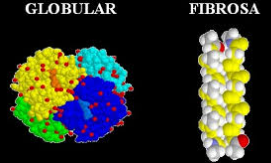
\includegraphics[width=0.45\linewidth,height=\textheight,keepaspectratio]{globulares.png}
\end{center}
\end{frame}

\begin{frame}{Características principales}
\phantomsection\label{caracteruxedsticas-principales}
\begin{itemize}
\tightlist
\item
  Están formadas por una \textbf{cadena de aminoácidos} que se pliega en
  una forma tridimensional específica.
\item
  En la \textbf{superficie} tienen grupos \textbf{hidrofílicos} (que se
  llevan bien con el agua).
\item
  En el \textbf{interior} tienen grupos \textbf{hidrofóbicos} (que
  evitan el agua).
\item
  Cada proteína tiene una forma \textbf{única y exacta}, lo que le da su
  función específica.
\end{itemize}

\begin{columns}[T]
\begin{column}{0.33\linewidth}
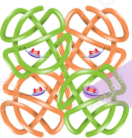
\includegraphics[width=0.7\linewidth,height=\textheight,keepaspectratio]{hemo.png}
\end{column}

\begin{column}{0.33\linewidth}
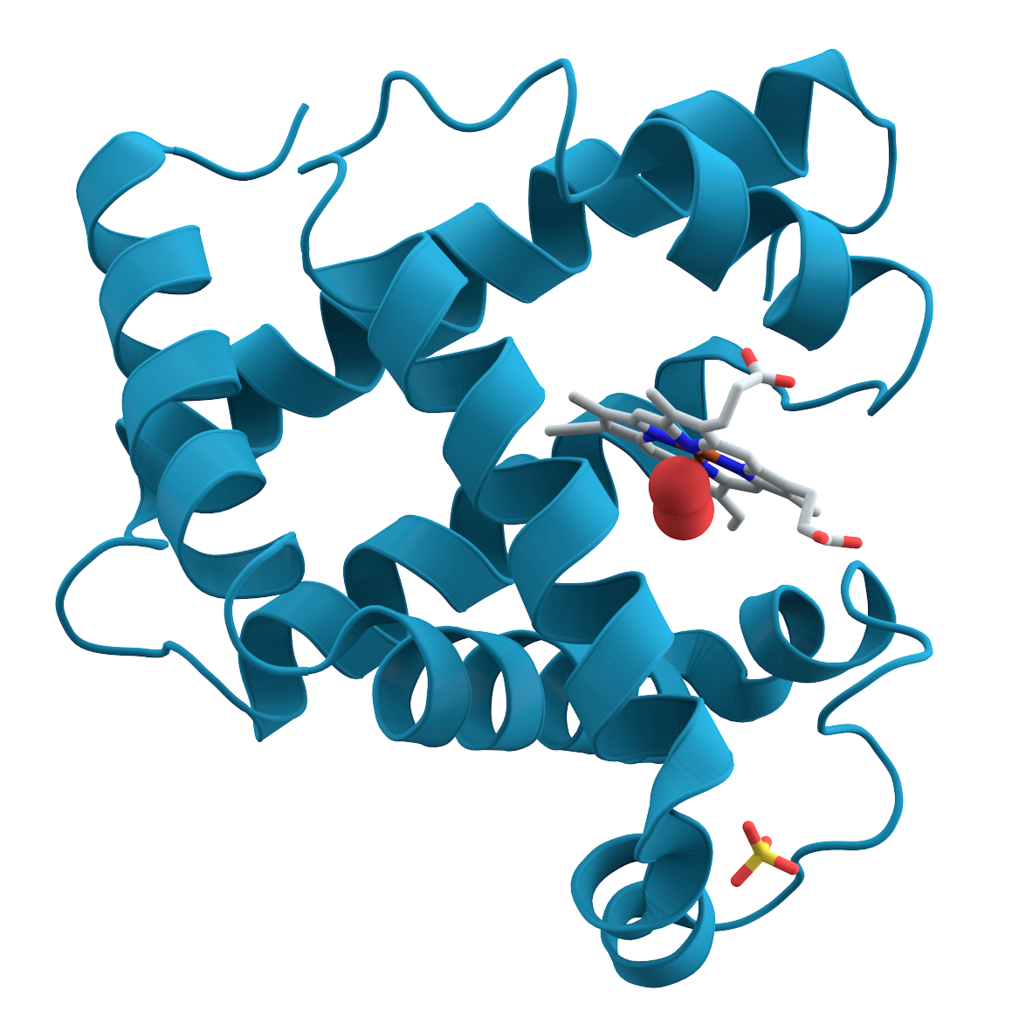
\includegraphics[width=0.7\linewidth,height=\textheight,keepaspectratio]{mioglobina.png}
\end{column}

\begin{column}{0.33\linewidth}
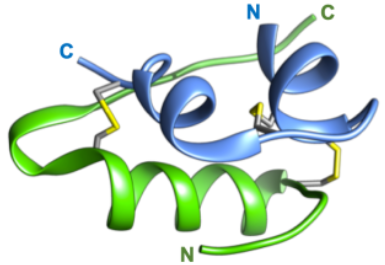
\includegraphics[width=0.7\linewidth,height=\textheight,keepaspectratio]{insulina.png}
\end{column}
\end{columns}
\end{frame}

\begin{frame}{Hemoglobina: la proteína que transporta oxígeno}
\phantomsection\label{hemoglobina-la-proteuxedna-que-transporta-oxuxedgeno}
\begin{itemize}
\tightlist
\item
  Es la \textbf{proteína encargada de llevar el oxígeno} en la sangre.
\item
  Se encuentra \textbf{dentro de los glóbulos rojos}.
\item
  Hay aproximadamente \textbf{15 g de hemoglobina por cada 100 ml de
  sangre}.
\item
  Su función es \textbf{tomar oxígeno en los pulmones} y
  \textbf{liberarlo en los tejidos} donde se necesita.
\end{itemize}

\begin{center}
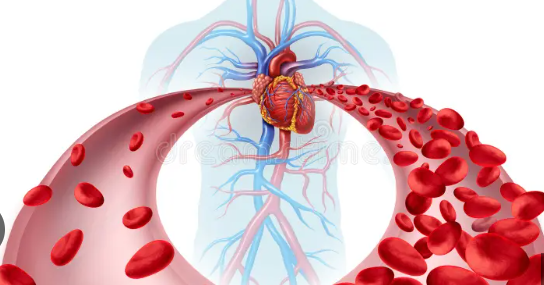
\includegraphics[width=0.45\linewidth,height=\textheight,keepaspectratio]{pulmon.png}
\end{center}
\end{frame}

\begin{frame}{¿De qué está hecha la hemoglobina?}
\phantomsection\label{de-quuxe9-estuxe1-hecha-la-hemoglobina}
La hemoglobina está formada por:

\begin{itemize}
\tightlist
\item
  \textbf{4 cadenas de globina} (proteínas)
\item
  \textbf{4 grupos hemo}, uno en cada cadena
\item
  Cada grupo hemo tiene un átomo de \textbf{hierro (Fe²⁺)} en el centro
\end{itemize}

Ese hierro es el que se \textbf{une al oxígeno}, por eso el
\textbf{hierro en la dieta es tan importante} 🩸

\begin{center}
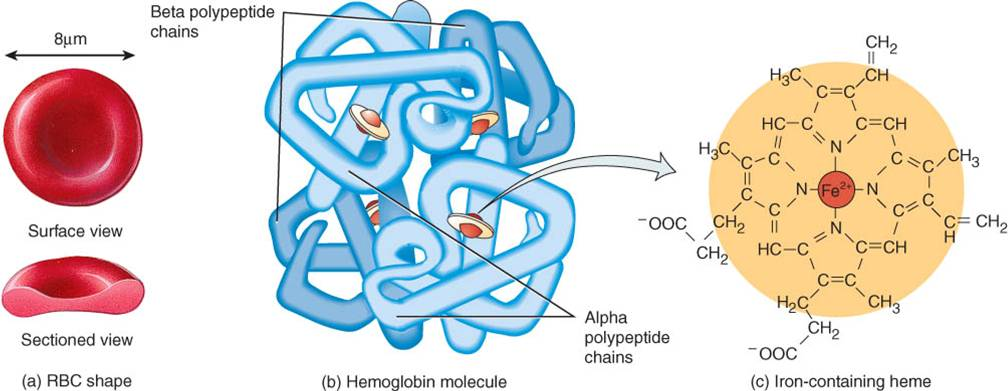
\includegraphics[width=0.45\linewidth,height=\textheight,keepaspectratio]{hemoglobina.jpg}
\end{center}
\end{frame}

\begin{frame}{Estructura de la hemoglobina (cómo está armada)}
\phantomsection\label{estructura-de-la-hemoglobina-cuxf3mo-estuxe1-armada}
\begin{itemize}
\tightlist
\item
  \textbf{Estructura primaria:} la secuencia de aminoácidos (como letras
  en una palabra).\\
\item
  \textbf{Estructura secundaria:} se forman espirales llamadas hélices
  alfa.\\
\item
  \textbf{Estructura terciaria:} cada cadena se pliega sobre sí misma.\\
\item
  \textbf{Estructura cuaternaria:} cuatro cadenas (dos α y dos β) se
  unen formando un tetrámero.
\end{itemize}

En total, son \textbf{cuatro subunidades que trabajan en equipo}.

\begin{center}
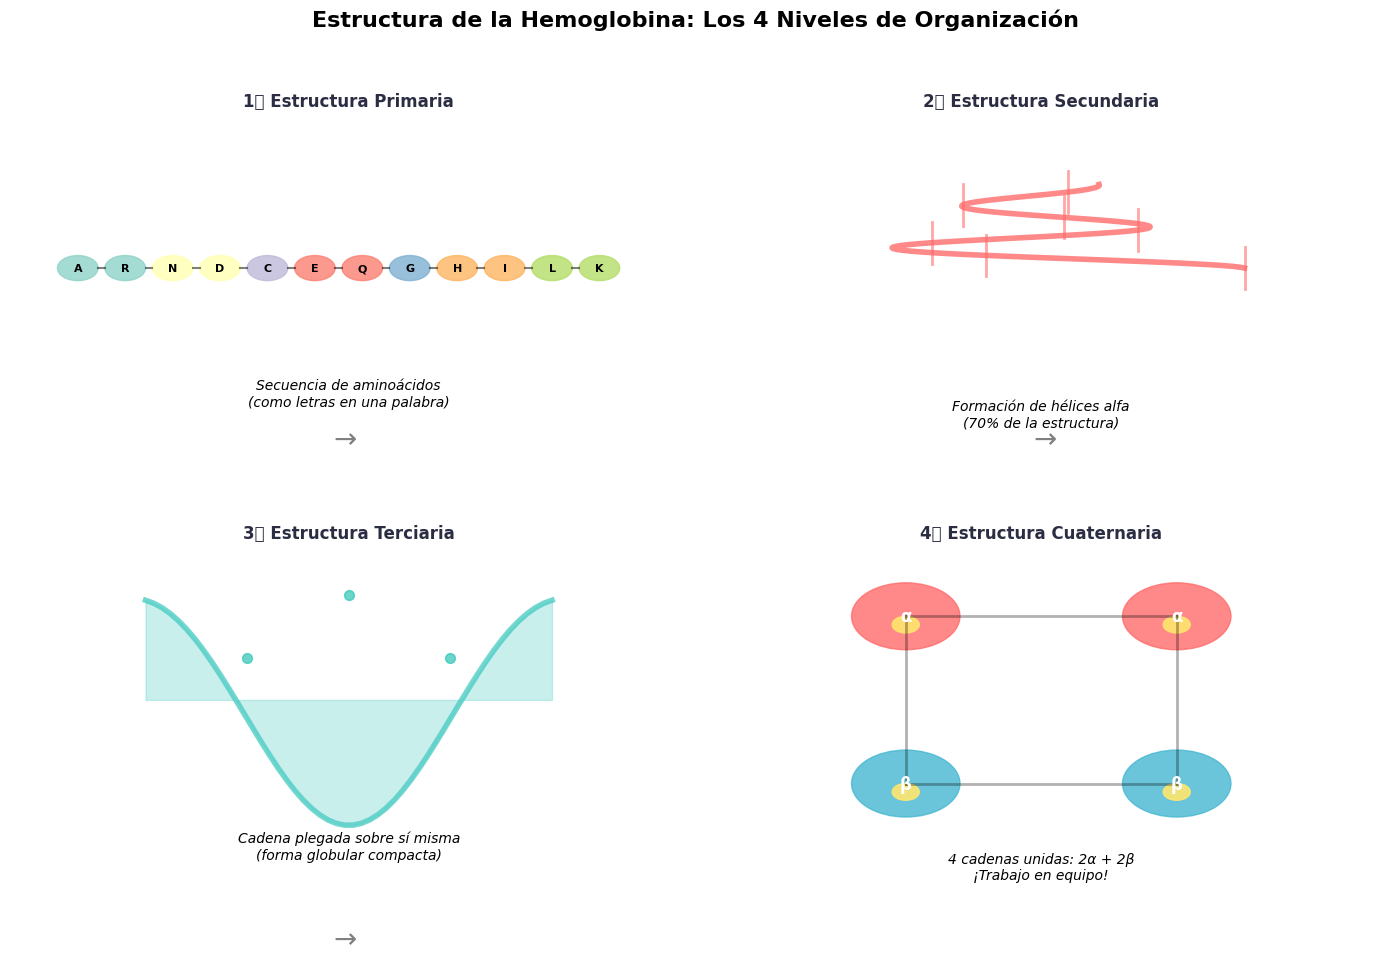
\includegraphics[width=0.4\linewidth,height=\textheight,keepaspectratio]{estructura.png}
\end{center}
\end{frame}

\begin{frame}{El grupo hemo: el corazón de la hemoglobina ❤️}
\phantomsection\label{el-grupo-hemo-el-corazuxf3n-de-la-hemoglobina}
\begin{itemize}
\tightlist
\item
  Es una molécula especial dentro de cada subunidad.\\
\item
  Tiene un \textbf{anillo de porfirina} con un \textbf{hierro ferroso
  (Fe²⁺)} en el centro.\\
\item
  El oxígeno se \textbf{une temporalmente} a ese hierro.\\
\item
  Si el hierro se oxida a Fe³⁺, ya \textbf{no puede unirse al oxígeno}.
\end{itemize}

Cuando la sangre está oxigenada → \textbf{roja brillante}\\
Cuando no lo está → \textbf{roja oscura o azulada}

\begin{columns}[T]
\begin{column}{0.5\linewidth}
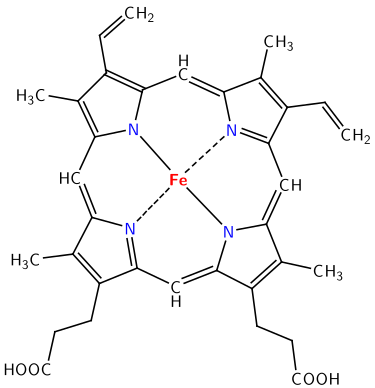
\includegraphics[width=0.65\linewidth,height=\textheight,keepaspectratio]{grupo.png}
\end{column}

\begin{column}{0.5\linewidth}
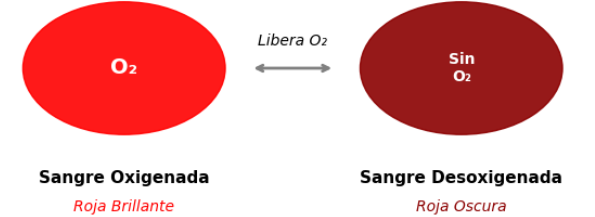
\includegraphics[width=0.6\linewidth,height=\textheight,keepaspectratio]{oxigenada.png}
\end{column}
\end{columns}
\end{frame}

\begin{frame}{Cómo funciona la hemoglobina 🫁➡️🫀➡️🦵}
\phantomsection\label{cuxf3mo-funciona-la-hemoglobina}
\begin{itemize}
\tightlist
\item
  La hemoglobina \textbf{capta oxígeno en los pulmones}, donde hay mucho
  O₂.\\
\item
  Luego \textbf{lo libera en los tejidos}, donde hay poco oxígeno.\\
\item
  Esta unión es \textbf{reversible}: puede unirse y soltar el oxígeno
  según se necesite.
\end{itemize}

``Funciona como un camión repartidor: carga oxígeno en los pulmones y lo
entrega donde hace falta.''

\begin{center}
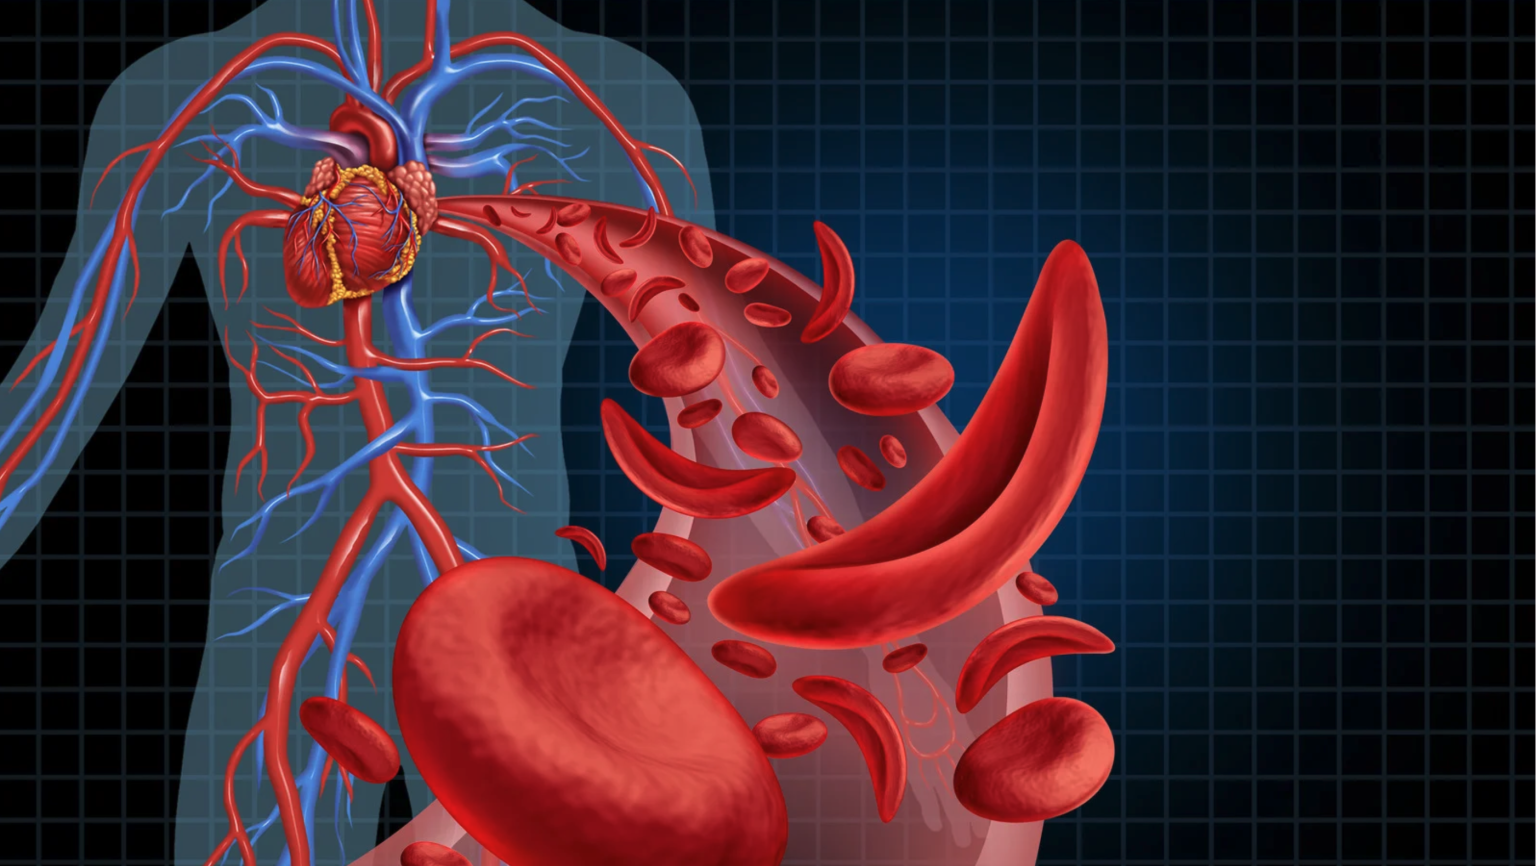
\includegraphics[width=0.45\linewidth,height=\textheight,keepaspectratio]{dispersion.png}
\end{center}
\end{frame}

\begin{frame}{Curva de disociación del oxígeno}
\phantomsection\label{curva-de-disociaciuxf3n-del-oxuxedgeno}
Representa qué tanto oxígeno está unido a la hemoglobina según la
cantidad disponible (presión parcial de O₂).

\begin{itemize}
\tightlist
\item
  La curva tiene forma de \textbf{S (sigmoide)}.\\
\item
  Esto significa que \textbf{cuanto más oxígeno se une, más fácil es que
  se una el siguiente}.\\
\item
  Este comportamiento se llama \textbf{cooperatividad}.
\end{itemize}

``La primera molécula de oxígeno entra con dificultad, pero las
siguientes se unen con más facilidad.''

\begin{center}
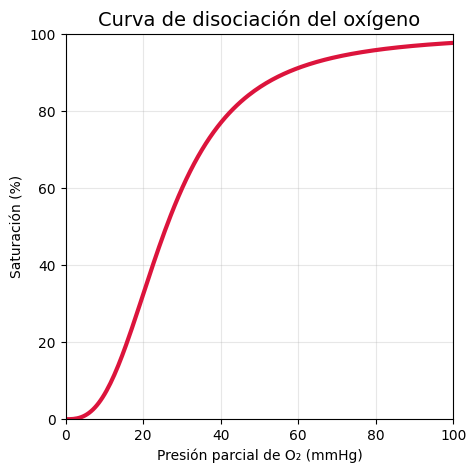
\includegraphics[width=0.3\linewidth,height=\textheight,keepaspectratio]{disociacion.png}
\end{center}
\end{frame}

\begin{frame}{Estados T y R: los ``modos'' de la hemoglobina}
\phantomsection\label{estados-t-y-r-los-modos-de-la-hemoglobina}
\begin{itemize}
\tightlist
\item
  \textbf{Estado T (Tenso):} baja afinidad por el oxígeno (le cuesta
  unirse).\\
\item
  \textbf{Estado R (Relajado):} alta afinidad (se une fácilmente).
\end{itemize}

Cuando una subunidad se une al O₂, \textbf{toda la molécula cambia de
forma}, pasando del estado T al R.

💬 ``Es como si la hemoglobina cambiara de forma para abrazar mejor al
oxígeno.''

\begin{center}
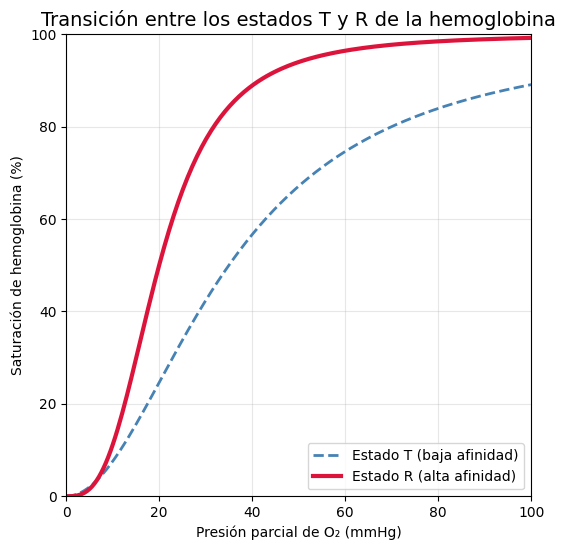
\includegraphics[width=0.3\linewidth,height=\textheight,keepaspectratio]{TR.png}
\end{center}
\end{frame}

\begin{frame}{Regulación: cómo el cuerpo controla la afinidad}
\phantomsection\label{regulaciuxf3n-cuxf3mo-el-cuerpo-controla-la-afinidad}
Factores que hacen que la hemoglobina \textbf{libere oxígeno más
fácilmente}:

\begin{itemize}
\tightlist
\item
  \textbf{2,3-BPG:} disminuye la afinidad → ayuda a soltar O₂ en
  tejidos.\\
\item
  \textbf{CO₂ y H⁺ (pH bajo):} facilitan que libere oxígeno →
  \emph{Efecto Bohr}.\\
\item
  \textbf{Temperatura alta:} también reduce la afinidad (en músculos
  calientes libera más O₂).
\end{itemize}

💡 En resumen:

\begin{itemize}
\tightlist
\item
  En los \textbf{pulmones} (pH alto, temperatura baja) → toma oxígeno.\\
\item
  En los \textbf{tejidos} (pH bajo, temperatura alta) → lo suelta.
\end{itemize}

\begin{center}
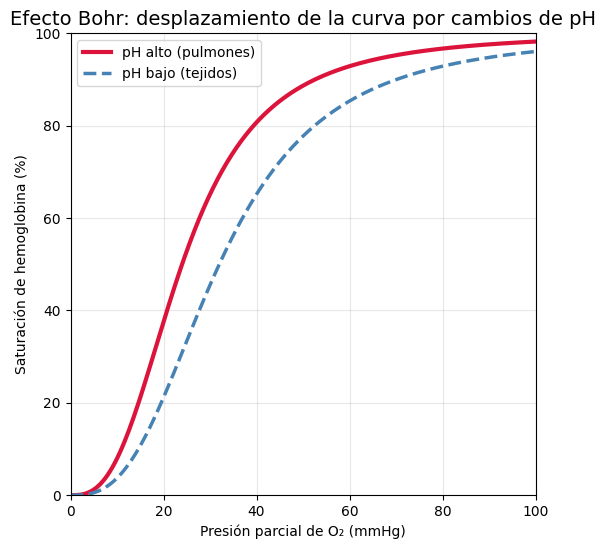
\includegraphics[width=0.3\linewidth,height=\textheight,keepaspectratio]{PH.png}
\end{center}
\end{frame}

\begin{frame}{✅ Conclusiones}
\phantomsection\label{conclusiones}
\begin{itemize}
\tightlist
\item
  La hemoglobina es una \textbf{proteína globular esencial} para la
  vida.\\
\item
  Su estructura permite un \textbf{mecanismo cooperativo} de unión al
  oxígeno.\\
\item
  Factores como el \textbf{pH, CO₂ y temperatura} regulan su función.\\
\item
  Gracias a ella, \textbf{el oxígeno llega justo donde el cuerpo lo
  necesita}.
\end{itemize}

\begin{center}
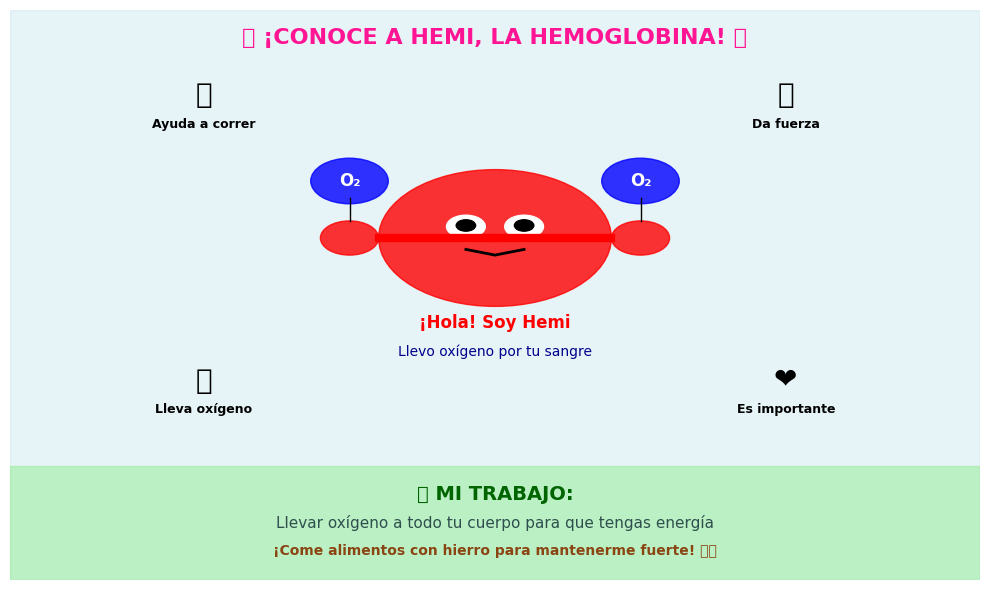
\includegraphics[width=0.55\linewidth,height=\textheight,keepaspectratio]{conclusion.png}
\end{center}
\end{frame}




\end{document}
